\section{Final Tables}
The summarized results are presented in three tables: 
\begin{itemize}
\item Table~\ref{tab:fourLeptonResults} contains observed yields  and background prediction 
for each search region in the four lepton channels
\end{itemize}

The graphical representation of the results is shown in Figures~\ref{fig:L4OSSF0tau0},~\ref{fig:L4OSSF0tau1},~\ref{fig:L4OSSF1offZtau0},~\ref{fig:L4OSSF1onZtau0},~\ref{fig:L4OSSF1offZtau1},~\ref{fig:L4OSSF1onZtau1},~\ref{fig:L4OSSF2offZtau0}, and~\ref{fig:L4OSSF2onZtau0}.

%==========================================================================================
\begin{figure}[htp]
\begin{center}
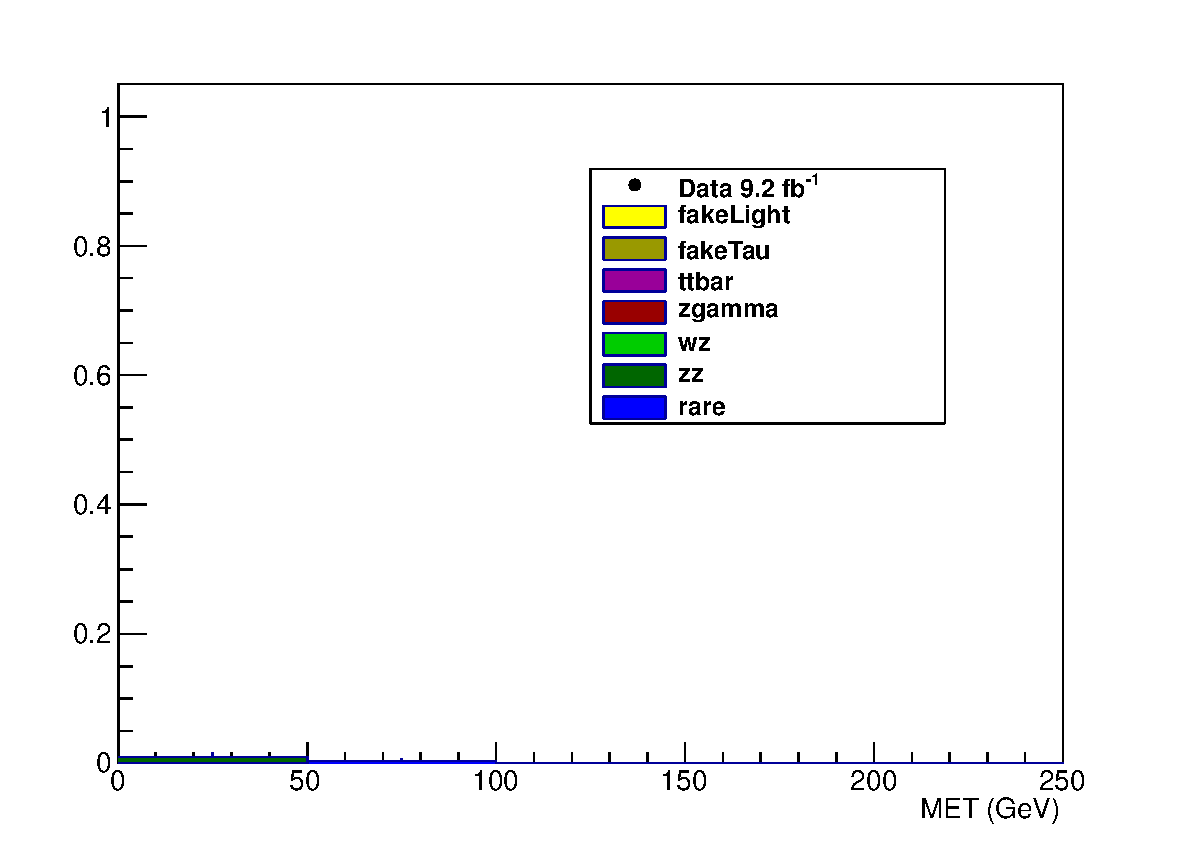
\includegraphics[width=1.0\textwidth]{plots/4L_MET_dist_offZ_ossf0_tau0_note.pdf}
\caption{Observed yields and predicted backgrounds for four lepton events with no OSSF pairs and zero taus.}
\label{fig:L4OSSF0tau0}
\end{center}
\end{figure}
%==========================================================================================

%==========================================================================================
\begin{figure}[htp]
\begin{center}
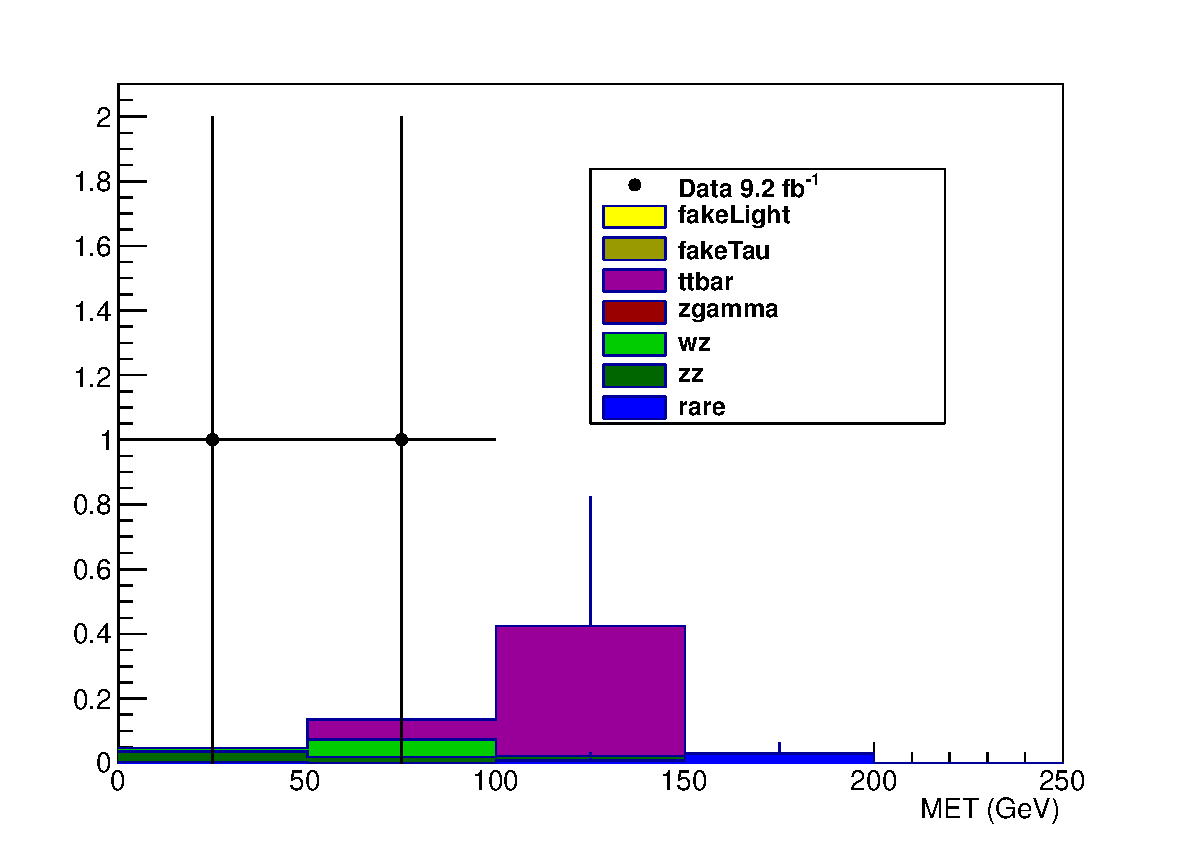
\includegraphics[width=1.0\textwidth]{plots/4L_MET_dist_offZ_ossf0_tau1_note.pdf}
\caption{Observed yields and predicted backgrounds for four lepton events with no OSSF pairs and one tau.}
\label{fig:L4OSSF0tau1}
\end{center}
\end{figure}
%==========================================================================================

%==========================================================================================
\begin{figure}[htp]
\begin{center}
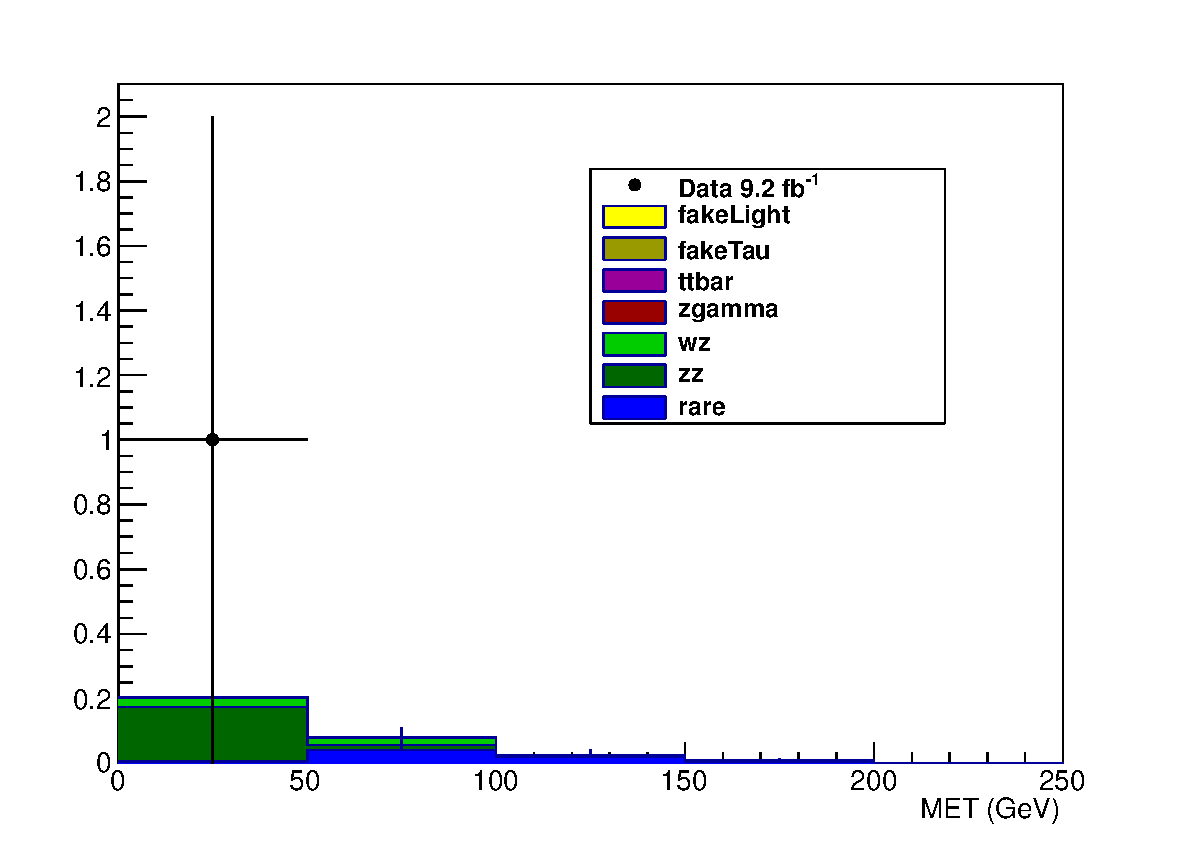
\includegraphics[width=1.0\textwidth]{plots/4L_MET_dist_offZ_ossf1_tau0_note.pdf}
\caption{Observed yields and predicted backgrounds for four lepton events with one OSSF pair offZ and zero taus.}
\label{fig:L4OSSF1offZtau0}
\end{center}
\end{figure}
%==========================================================================================

%==========================================================================================
\begin{figure}[htp]
\begin{center}
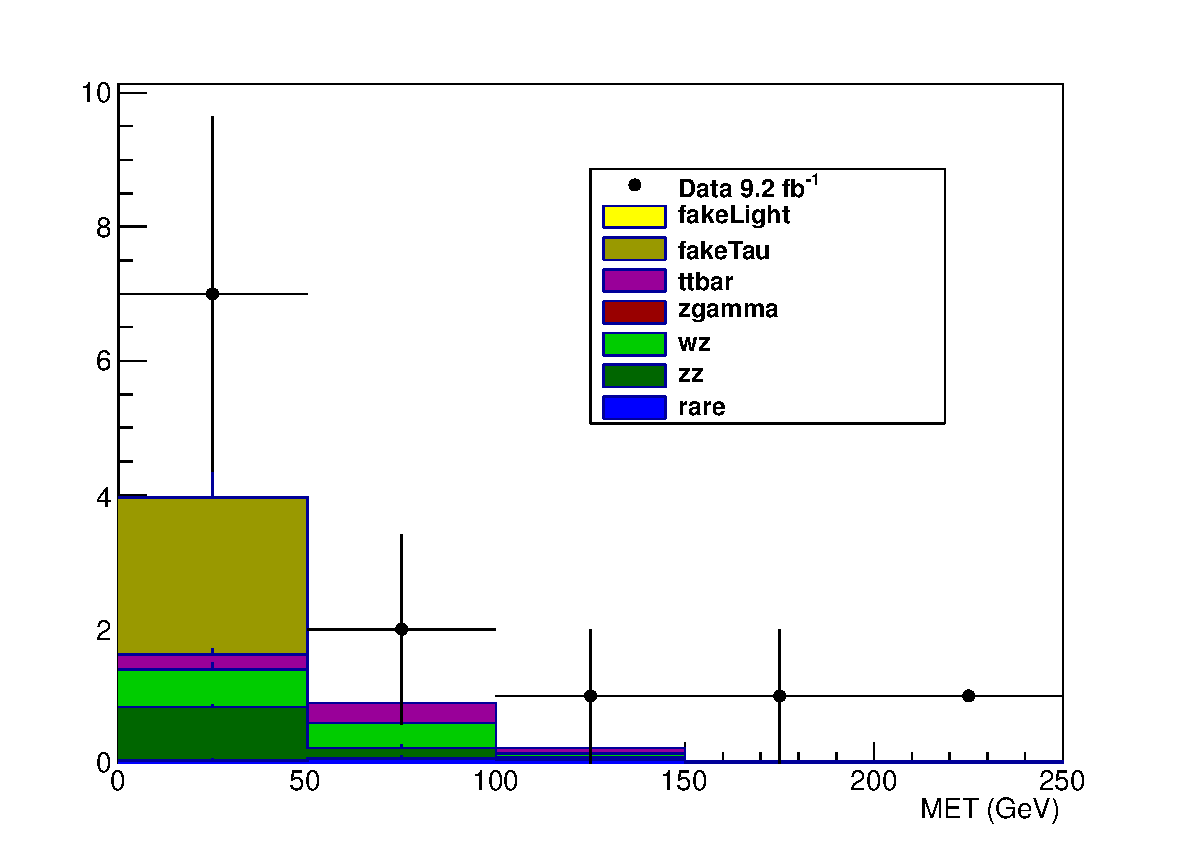
\includegraphics[width=1.0\textwidth]{plots/4L_MET_dist_offZ_ossf1_tau1_note.pdf}
\caption{Observed yields and predicted backgrounds for four lepton events with one OSSF pair off Z and one tau.}
\label{fig:L4OSSF1offZtau1}
\end{center}
\end{figure}
%==========================================================================================

%==========================================================================================
\begin{figure}[htp]
\begin{center}
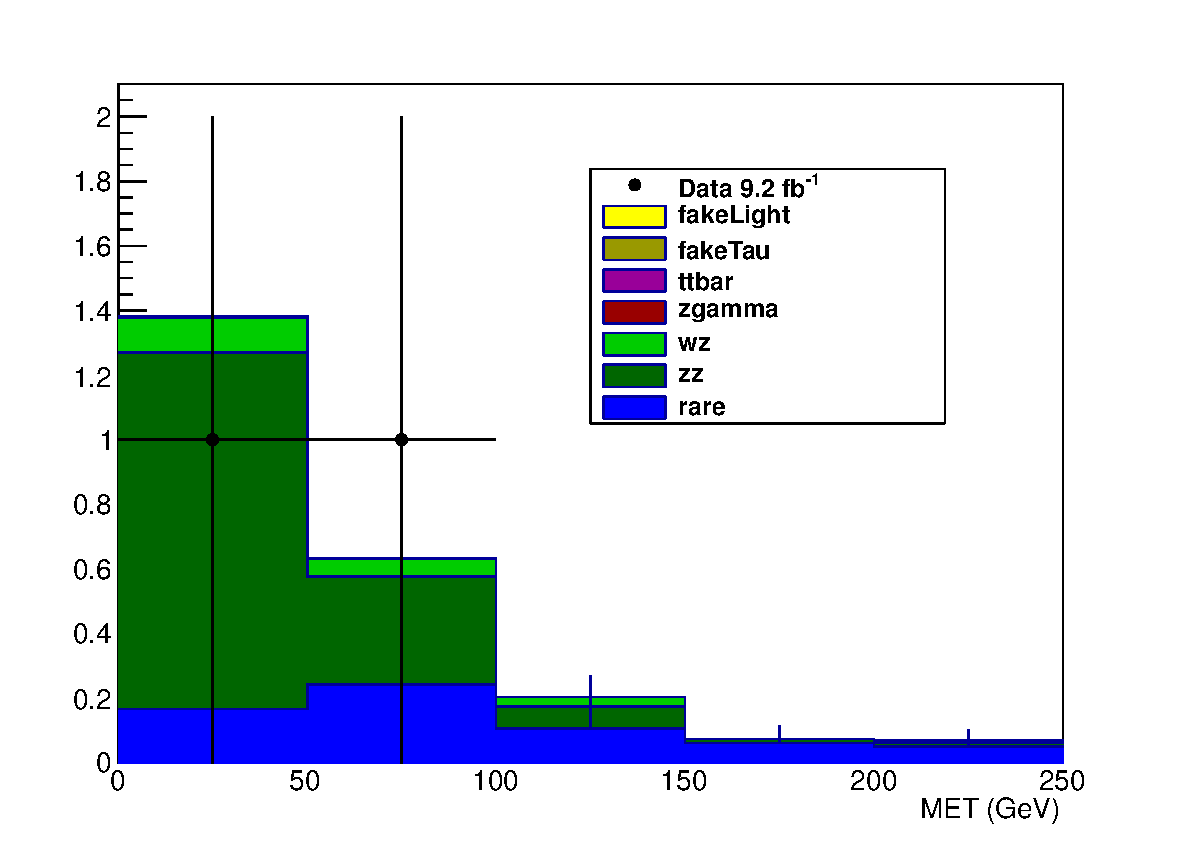
\includegraphics[width=1.0\textwidth]{plots/4L_MET_dist_onZ_ossf1_tau0_note.pdf}
\caption{Observed yields and predicted backgrounds for four lepton events with one OSSF pair on Z and zero taus.}
\label{fig:L4OSSF1onZtau0}
\end{center}
\end{figure}
%==========================================================================================

%==========================================================================================
\begin{figure}[htp]
\begin{center}
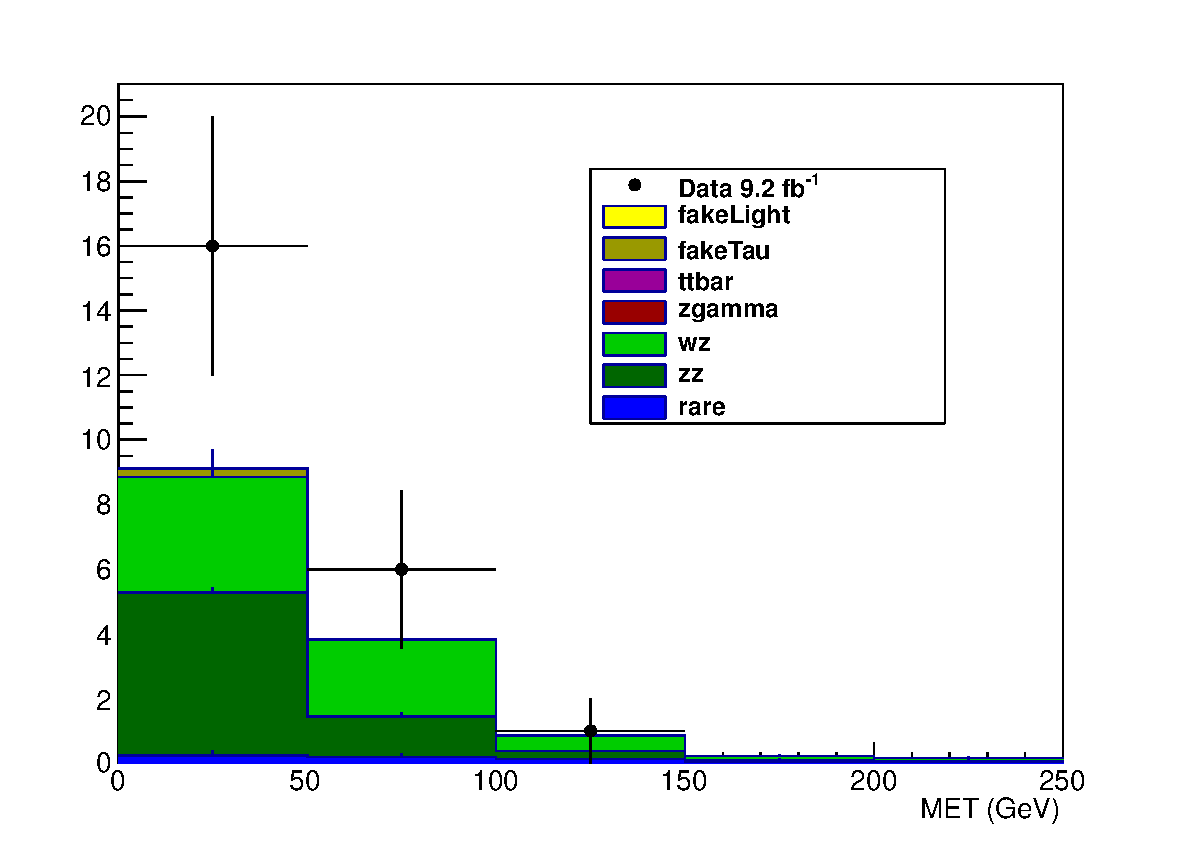
\includegraphics[width=1.0\textwidth]{plots/4L_MET_dist_onZ_ossf1_tau1_note.pdf}
\caption{Observed yields and predicted backgrounds for four lepton events with one OSSF pair on Z and one tau.}
\label{fig:L4OSSF1onZtau1}
\end{center}
\end{figure}
%==========================================================================================

%==========================================================================================
\begin{figure}[htp]
\begin{center}
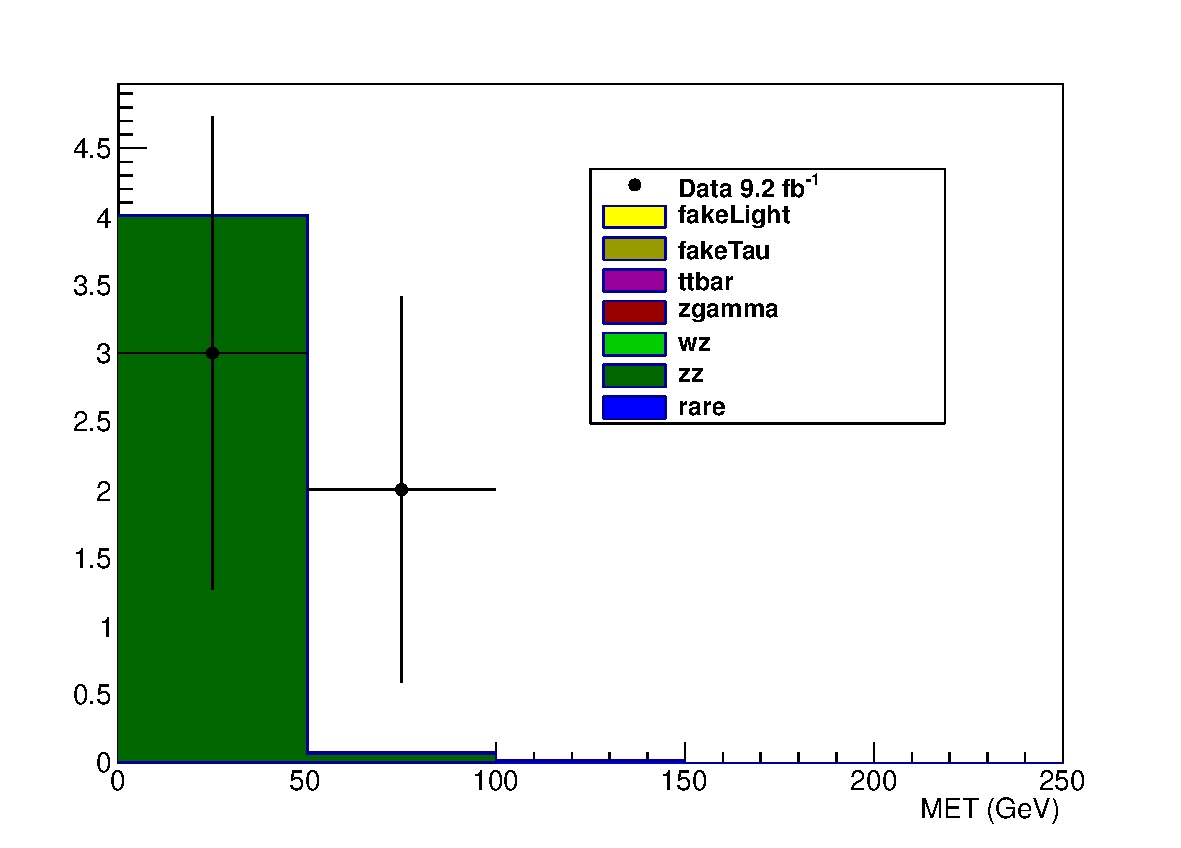
\includegraphics[width=1.0\textwidth]{plots/4L_MET_dist_offZ_ossf2_tau0_note.pdf}
\caption{Observed yields and predicted backgrounds for four lepton events with two OSSF pairs offZ and zero taus.}
\label{fig:L4OSSF2offZtau0}
\end{center}
\end{figure}
%==========================================================================================

%==========================================================================================
\begin{figure}[htp]
\begin{center}
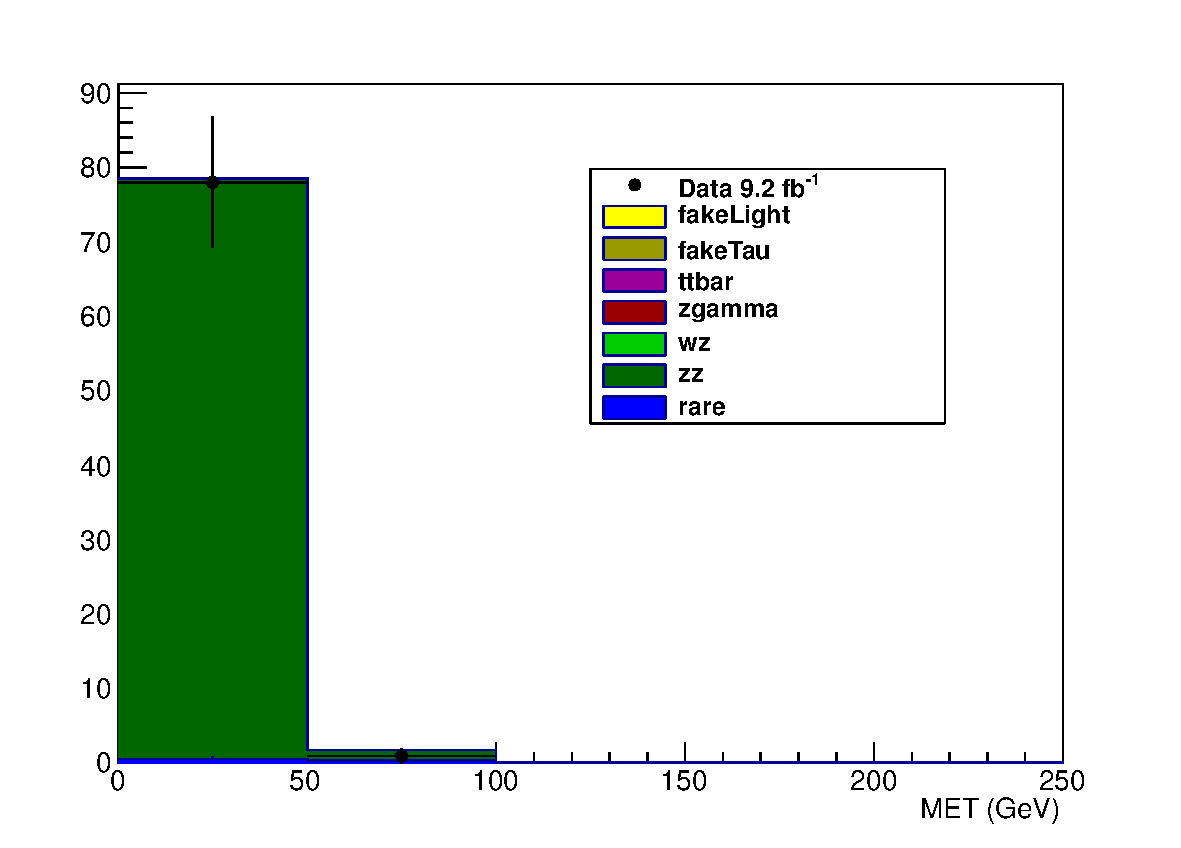
\includegraphics[width=1.0\textwidth]{plots/4L_MET_dist_onZ_ossf2_tau0_note.pdf}
\caption{Observed yields and predicted backgrounds for four lepton events with two OSSF pairs onZ and zero taus.}
\label{fig:L4OSSF2onZtau0}
\end{center}
\end{figure}
%==========================================================================================


\begin{sidewaystable}
\tiny
\begin{center}
\caption{\label{tab:fourLeptonResults} Four lepton backgrounds and observed yields}
\begin{tabular}{|c|cccccc|c|c|}
\hline
\hline
$\MET$ & WZ & $\TTbar$ &  Non-prompt & $Z\gamma^{*}$ & ZZ & Rare SM & Total Bkg & Observed \\
\hline
\hline
\hline
4L MET dist offZ ossf0 tau0\\
50--100 & 0.00 $\pm$ 0.00 & 0.00 $\pm$ 0.00 & 0.00 $\pm$ 0.00 & 0.00 $\pm$ 0.00 & 0.00 $\pm$ 0.00 & 0.00 $\pm$ 0.00 & 0.00 $\pm$ 0.00 & 0 \\
100--150 & 0.00 $\pm$ 0.00 & 0.00 $\pm$ 0.00 & 0.00 $\pm$ 0.00 & 0.00 $\pm$ 0.00 & 0.00 $\pm$ 0.00 & 0.00 $\pm$ 0.00 & 0.00 $\pm$ 0.00 & 0 \\
150--200 & 0.00 $\pm$ 0.00 & 0.00 $\pm$ 0.00 & 0.00 $\pm$ 0.00 & 0.00 $\pm$ 0.00 & 0.00 $\pm$ 0.00 & 0.00 $\pm$ 0.00 & 0.00 $\pm$ 0.00 & 0 \\
200--250 & 0.00 $\pm$ 0.00 & 0.00 $\pm$ 0.00 & 0.00 $\pm$ 0.00 & 0.00 $\pm$ 0.00 & 0.00 $\pm$ 0.00 & 0.00 $\pm$ 0.00 & 0.00 $\pm$ 0.00 & 0 \\
\hline
4L MET dist offZ ossf0 tau1\\
50--100 & 0.05 $\pm$ 0.02 & 0.06 $\pm$ 0.06 & 0.00 $\pm$ 0.00 & 0.00 $\pm$ 0.00 & 0.02 $\pm$ 0.01 & 0.00 $\pm$ 0.00 & 0.13 $\pm$ 0.06 & 1 \\
100--150 & 0.00 $\pm$ 0.00 & 0.40 $\pm$ 0.40 & 0.00 $\pm$ 0.00 & 0.00 $\pm$ 0.00 & 0.02 $\pm$ 0.01 & 0.01 $\pm$ 0.01 & 0.42 $\pm$ 0.40 & 0 \\
150--200 & 0.00 $\pm$ 0.00 & 0.00 $\pm$ 0.00 & 0.00 $\pm$ 0.00 & 0.00 $\pm$ 0.00 & 0.00 $\pm$ 0.00 & 0.03 $\pm$ 0.03 & 0.03 $\pm$ 0.03 & 0 \\
200--250 & 0.00 $\pm$ 0.00 & 0.00 $\pm$ 0.00 & 0.00 $\pm$ 0.00 & 0.00 $\pm$ 0.00 & 0.00 $\pm$ 0.00 & 0.00 $\pm$ 0.00 & 0.00 $\pm$ 0.00 & 0 \\
\hline
4L MET dist offZ ossf1 tau0\\
50--100 & 0.02 $\pm$ 0.01 & 0.00 $\pm$ 0.00 & 0.00 $\pm$ 0.00 & 0.00 $\pm$ 0.00 & 0.02 $\pm$ 0.01 & 0.04 $\pm$ 0.03 & 0.08 $\pm$ 0.03 & 0 \\
100--150 & 0.00 $\pm$ 0.00 & 0.00 $\pm$ 0.00 & 0.00 $\pm$ 0.00 & 0.00 $\pm$ 0.00 & 0.00 $\pm$ 0.00 & 0.02 $\pm$ 0.02 & 0.02 $\pm$ 0.02 & 0 \\
150--200 & 0.00 $\pm$ 0.00 & 0.00 $\pm$ 0.00 & 0.00 $\pm$ 0.00 & 0.00 $\pm$ 0.00 & 0.01 $\pm$ 0.01 & 0.00 $\pm$ 0.00 & 0.01 $\pm$ 0.01 & 0 \\
200--250 & 0.00 $\pm$ 0.00 & 0.00 $\pm$ 0.00 & 0.00 $\pm$ 0.00 & 0.00 $\pm$ 0.00 & 0.00 $\pm$ 0.00 & 0.00 $\pm$ 0.00 & 0.00 $\pm$ 0.00 & 0 \\
\hline
4L MET dist offZ ossf1 tau1\\
50--100 & 0.36 $\pm$ 0.06 & 0.30 $\pm$ 0.04 & 0.00 $\pm$ 0.00 & 0.00 $\pm$ 0.00 & 0.15 $\pm$ 0.03 & 0.06 $\pm$ 0.04 & 0.86 $\pm$ 0.09 & 2 \\
100--150 & 0.06 $\pm$ 0.02 & 0.08 $\pm$ 0.02 & 0.00 $\pm$ 0.00 & 0.00 $\pm$ 0.00 & 0.03 $\pm$ 0.01 & 0.04 $\pm$ 0.03 & 0.22 $\pm$ 0.04 & 1 \\
150--200 & 0.00 $\pm$ 0.00 & 0.01 $\pm$ 0.01 & 0.00 $\pm$ 0.00 & 0.00 $\pm$ 0.00 & 0.01 $\pm$ 0.00 & 0.00 $\pm$ 0.00 & 0.02 $\pm$ 0.01 & 1 \\
200--250 & 0.01 $\pm$ 0.00 & 0.00 $\pm$ 0.00 & 0.00 $\pm$ 0.00 & 0.00 $\pm$ 0.00 & 0.00 $\pm$ 0.00 & 0.01 $\pm$ 0.01 & 0.02 $\pm$ 0.01 & 1 \\
\hline
4L MET dist offZ ossf2 tau0\\
50--100 & 0.01 $\pm$ 0.00 & 0.00 $\pm$ 0.00 & 0.00 $\pm$ 0.00 & 0.00 $\pm$ 0.00 & 0.05 $\pm$ 0.01 & 0.00 $\pm$ 0.00 & 0.06 $\pm$ 0.01 & 2 \\
100--150 & 0.00 $\pm$ 0.00 & 0.00 $\pm$ 0.00 & 0.00 $\pm$ 0.00 & 0.00 $\pm$ 0.00 & 0.01 $\pm$ 0.01 & 0.01 $\pm$ 0.01 & 0.02 $\pm$ 0.01 & 0 \\
150--200 & 0.00 $\pm$ 0.00 & 0.00 $\pm$ 0.00 & 0.00 $\pm$ 0.00 & 0.00 $\pm$ 0.00 & 0.00 $\pm$ 0.00 & 0.00 $\pm$ 0.00 & 0.00 $\pm$ 0.00 & 0 \\
200--250 & 0.00 $\pm$ 0.00 & 0.00 $\pm$ 0.00 & 0.00 $\pm$ 0.00 & 0.00 $\pm$ 0.00 & 0.00 $\pm$ 0.00 & 0.00 $\pm$ 0.00 & 0.00 $\pm$ 0.00 & 0 \\
\hline
4L MET dist onZ ossf1 tau0\\
50--100 & 0.06 $\pm$ 0.02 & 0.00 $\pm$ 0.00 & 0.00 $\pm$ 0.00 & 0.00 $\pm$ 0.00 & 0.33 $\pm$ 0.04 & 0.24 $\pm$ 0.14 & 0.63 $\pm$ 0.14 & 1 \\
100--150 & 0.03 $\pm$ 0.01 & 0.00 $\pm$ 0.00 & 0.00 $\pm$ 0.00 & 0.00 $\pm$ 0.00 & 0.07 $\pm$ 0.02 & 0.11 $\pm$ 0.06 & 0.20 $\pm$ 0.07 & 0 \\
150--200 & 0.00 $\pm$ 0.00 & 0.00 $\pm$ 0.00 & 0.00 $\pm$ 0.00 & 0.00 $\pm$ 0.00 & 0.01 $\pm$ 0.01 & 0.06 $\pm$ 0.04 & 0.07 $\pm$ 0.04 & 0 \\
200--250 & 0.01 $\pm$ 0.00 & 0.00 $\pm$ 0.00 & 0.00 $\pm$ 0.00 & 0.00 $\pm$ 0.00 & 0.01 $\pm$ 0.01 & 0.05 $\pm$ 0.03 & 0.07 $\pm$ 0.03 & 0 \\
\hline
4L MET dist onZ ossf1 tau1\\
50--100 & 2.36 $\pm$ 0.34 & 0.00 $\pm$ 0.00 & 0.00 $\pm$ 0.00 & 0.00 $\pm$ 0.00 & 1.31 $\pm$ 0.08 & 0.14 $\pm$ 0.08 & 3.81 $\pm$ 0.36 & 6 \\
100--150 & 0.48 $\pm$ 0.07 & 0.00 $\pm$ 0.00 & 0.00 $\pm$ 0.00 & 0.00 $\pm$ 0.00 & 0.29 $\pm$ 0.04 & 0.13 $\pm$ 0.08 & 0.89 $\pm$ 0.11 & 1 \\
150--200 & 0.12 $\pm$ 0.03 & 0.00 $\pm$ 0.00 & 0.00 $\pm$ 0.00 & 0.00 $\pm$ 0.00 & 0.06 $\pm$ 0.01 & 0.04 $\pm$ 0.03 & 0.22 $\pm$ 0.04 & 0 \\
200--250 & 0.08 $\pm$ 0.02 & 0.00 $\pm$ 0.00 & 0.00 $\pm$ 0.00 & 0.00 $\pm$ 0.00 & 0.01 $\pm$ 0.01 & 0.04 $\pm$ 0.02 & 0.13 $\pm$ 0.03 & 0 \\
\hline
4L MET dist onZ ossf2 tau0\\
50--100 & 0.03 $\pm$ 0.01 & 0.00 $\pm$ 0.00 & 0.00 $\pm$ 0.00 & 0.00 $\pm$ 0.00 & 1.42 $\pm$ 0.07 & 0.32 $\pm$ 0.18 & 1.77 $\pm$ 0.19 & 1 \\
100--150 & 0.01 $\pm$ 0.00 & 0.00 $\pm$ 0.00 & 0.00 $\pm$ 0.00 & 0.00 $\pm$ 0.00 & 0.08 $\pm$ 0.02 & 0.09 $\pm$ 0.05 & 0.17 $\pm$ 0.05 & 0 \\
150--200 & 0.00 $\pm$ 0.00 & 0.00 $\pm$ 0.00 & 0.00 $\pm$ 0.00 & 0.00 $\pm$ 0.00 & 0.03 $\pm$ 0.01 & 0.06 $\pm$ 0.04 & 0.09 $\pm$ 0.04 & 0 \\
200--250 & 0.00 $\pm$ 0.00 & 0.00 $\pm$ 0.00 & 0.00 $\pm$ 0.00 & 0.00 $\pm$ 0.00 & 0.02 $\pm$ 0.01 & 0.06 $\pm$ 0.04 & 0.08 $\pm$ 0.04 & 0 \\
\hline
\hline
\end{tabular}
\end{center}
\end{sidewaystable}